\documentclass[10pt]{article}
\usepackage[utf8]{inputenc}
\usepackage[T1]{fontenc}
\usepackage{lmodern}
\usepackage{listings}
\usepackage{makeidx}
\usepackage[toc, page]{appendix}
\usepackage{float}
\usepackage{lscape}
\usepackage{csquotes}
\usepackage{soul}
\usepackage{textcomp}
\usepackage{gensymb}
\usepackage{pdfpages}
\usepackage{caption}
\usepackage{subcaption}
\usepackage{url}
\lstset{
	keywords={SELECT, WHERE, COLUMNS, ROWS, ON, MEMBER, WITH, FROM, ALL, CROSSJOIN, TOPCOUNT, ASC, DESC, AS, PARENT, CURRENTMEMBER, CHILDREN, PREVMEMBER, NEXTMEMBER, ORDER, RANK, GENERATE},
	keywordstyle=\color{red}\bfseries
}
% \usepackage{geometry}
\usepackage[left=20mm, right=20mm, top=25mm, bottom=25mm]{geometry}
\usepackage{rotating}
\usepackage[section]{placeins}
\usepackage{chngcntr,array}
\usepackage{graphicx}
\usepackage{lscape}
\usepackage{dirtree}
\usepackage[
	breaklinks=true,
	colorlinks=true,
	linkcolor=blue,
	urlcolor=blue,
	citecolor=blue,
	bookmarks=true,
	bookmarksopenlevel=2
]{hyperref}
\usepackage{xcolor}
\usepackage{algorithm}
\usepackage{algpseudocode}
\usepackage{amsmath}
\usepackage{amsfonts}
\usepackage{amssymb}
\usepackage{indentfirst}

\title{
	Machine Learning
	\\-\\
	Supervised Learning
}
\author{
	\href{mailto:brandon.alves@gatech.edu}{Brandon Alves}
}
\date{\today}

\begin{document}
	\maketitle
	\thispagestyle{empty}
	\tableofcontents
	% \listoffigures
	% \clearpage
	% \setcounter{page}{1}
	\section{Introduction}
		Optimisation is the goal of finding the best state over an input space, with respect to a fitness function. In this article, I will explore four different Randomised Optimisers on three different problems. I will be using the following optimisers:
		\begin{itemize}
			\item Random Hill Climbing
			\item Simulated Annealing
			\item Genetic Algorithm
			\item MIMIC
		\end{itemize}
		I will discuss their performance and compare them to each other. I will also discuss the pros and cons of each optimiser depending on the problem. In that purpose, I will explore multiple meta-parameters for each optimiser. I will use those optimisers on the following problems:
		\begin{itemize}
			\item Traveling Salesman
			\item Flip Flop
			\item Four Peaks
		\end{itemize}
		I will also use the three first optimisers to find good weights for a neural network on the credit card fraud dataset. Like in the previous report, the graphs presented in this report follow the same format. The hard line represents the median value while the hue areas fill the space between the minimal and maximal values.
	\section{Random Optimisation}
		\subsection{Traveling Salesman Problem}
			\subsubsection*{Introduction}
				The Traveling Salesman Problem (TSP) is a well-known problem in the field of optimisation. It consists in finding the shortest path that visits all the cities of a given graph. The TSP is a NP-hard problem, which means that it is difficult to solve. In this section, we will present the results of the optimisers on the TSP problem.
				For this problem, the fitness function to minimise is the length of the path:
				\begin{equation}
					f(d) = \frac{1}{d}
				\end{equation}
				with $d$ the length of the path.
				We present on figure \ref{tsp:all} the results of the four different optimisers on the TSP problem. The first thing to notice is that there is a lot of variation for each algorithm. RHC and SA have an median accuracy which are pretty close. GA does a little bit better while MIMIC gets the best median result. We can also notice that MIMIC gets the best results with a low number of iteration and reaches its bets optimisation only after a few iterations.
				\begin{figure}[h]
					\centering
					\begin{subfigure}[t]{0.45\columnwidth}
						\centering
						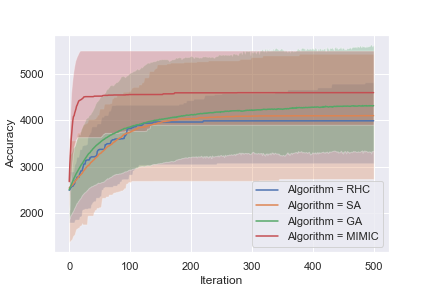
\includegraphics[width=\linewidth]{../graphics/tsp_all_Iteration_Error_Algorithm.png}
						\caption{Accuracy on TSP Problem for the different algorithms}
						\label{tsp:all_accuracy}
					\end{subfigure}
					% ~
					\begin{subfigure}[t]{0.45\columnwidth}
						\centering
						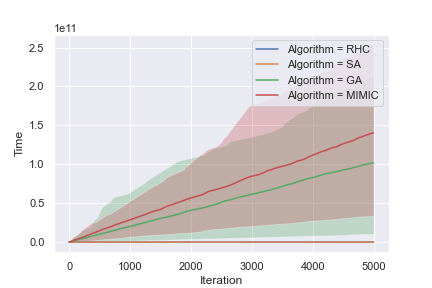
\includegraphics[width=\linewidth]{../graphics/tsp_all_Iteration_Time_Algorithm.png}
						\caption{Time on TSP Problem for the different algorithms}
						\label{tsp:all_time}
					\end{subfigure}
					\caption{Accuracy and Time on TSP Problem for the different algorithms}
					\label{tsp:all}
				\end{figure}
			\subsubsection*{Randomised Hill Climbing}
				The only parameter we will discuss here for RHC is the number of iterations. We see that the number of iterations has an impact on the performance of the algorithm. The best results are obtained with a high number of iterations but RHC does not success to get a good accuracy even with a high number of iterations as we can see on figure \ref{tsp:all_accuracy}. It is not surprising that RHC does not get good results on this problem because it is a local optimiser. It will not be able to find the best solution because it will get stuck in a local optimum.

				RHC is the fastest algorithm of the four as we can see on figure \ref{tsp:all_time}. It is not surprising because it is a local optimiser and it does not explore the whole search space. It only exploit the neighbourhood of the current state.

				To conclude, RHC is not well suited for this problem even if we appreciate its speed.
			\subsubsection*{Simulated Annealing}
				SA gives the second worst median results on this problem. For SA, we will discuss the following parameters:
				\begin{itemize}
					\item Temperature
					\item Cooling Rate
				\end{itemize}

				\begin{figure}[h]
					\centering
					\begin{subfigure}[t]{0.45\columnwidth}
						\centering
						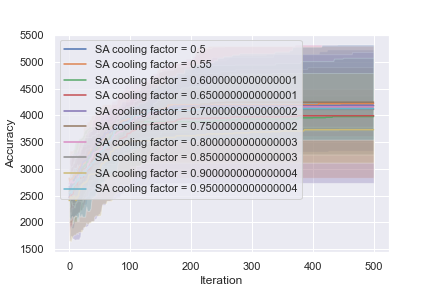
\includegraphics[width=\linewidth]{../graphics/tsp_SA_Iteration_Error_SA_cooling_factor.png}
						\caption{Accuracy on TSP with SA, for different cooling factors}
						\label{tsp:sa_cooling}
					\end{subfigure}
					~
					\begin{subfigure}[t]{0.45\columnwidth}
						\centering
						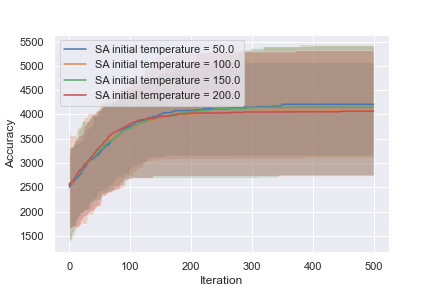
\includegraphics[width=1\linewidth]{../graphics/tsp_SA_Iteration_Error_SA_initial_temperature.png}
						\caption{Accuracy on TSP with SA, for different initial temperatures}
						\label{tsp:sa_initial_temp}
					\end{subfigure}
					\caption{Accuracy of SA on TSP according to Initial Temperature and Cooling Factor}
					\label{tsp:sa}
				\end{figure}

				We can see the inpact of the cooling factor on the accuracy of the algorithm on figure \ref{tsp:sa_cooling}. We notice that the cooling factor does not seem to be related to the algorithm.

				We can see the impact of the initial temperature on the accuracy of the algorithm on figure \ref{tsp:sa_initial_temp}. Like for the cooling factor, the initial temperature does not impact a lot the accuracy of the algorithm. The best results are obtained with a low initial temperature of 50.

				SA is the second fastest algorithm of the four as we can see on figure \ref{tsp:all_time}. It is not surprising because of its similarity with RHC.

				To conclude, as RHC, SA is not really well suited for this problem.
			\subsubsection*{Genetic Algorithm}
				GA gives the second best median results on this problem. Figure \ref{tsp:ga} shows the impact of the following parameters:
				\begin{itemize}
					\item Population Size
					\item Mutate Number
					\item Mate Number
				\end{itemize}

				\begin{figure}[h]
					\centering
					\begin{subfigure}[t]{0.32\columnwidth}
						\centering
						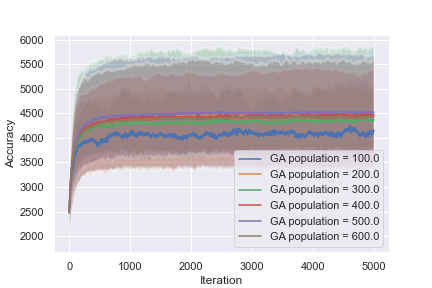
\includegraphics[width=\linewidth]{../graphics/tsp_GA_Iteration_Error_GA_population.png}
						\caption{Accuracy on TSP with GA, for different population size}
						\label{tsp:ga_pop}
					\end{subfigure}
					~
					\begin{subfigure}[t]{0.32\columnwidth}
						\centering
						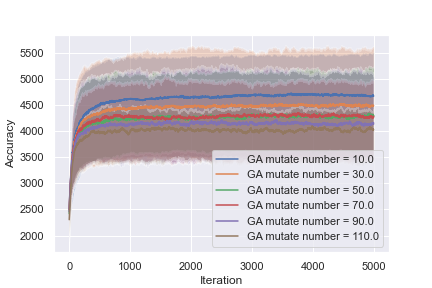
\includegraphics[width=\linewidth]{../graphics/tsp_GA_Iteration_Error_GA_mutate_number.png}
						\caption{Accuracy on TSP with GA, for different mutate number, with population set to 600}
						\label{tsp:ga_mutate}
					\end{subfigure}
					~
					\begin{subfigure}[t]{0.32\columnwidth}
						\centering
						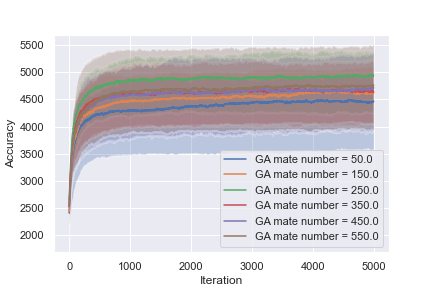
\includegraphics[width=\linewidth]{../graphics/tsp_GA_Iteration_Error_GA_mate_number.png}
						\caption{Accuracy on TSP with GA, for different mate number, with population set to 600 and mutate number to 10}
						\label{tsp:ga_mate}
					\end{subfigure}
					\caption{Accuracy of GA on TSP according to Population Size, Mutate Number and Mate Number}
					\label{tsp:ga}
				\end{figure}

				Let's start with the population size. We can see on figure \ref{tsp:ga_pop} that the accuracy is the highest for high values of population size while it is the lowest for low values of population size. We can see that the best results are obtained with a population size of 500. The fact that the accuracy depends on the population size is not surprising because the population size is the number of individuals in the population. The more individuals we have, the more chances we have to find a good solution.

				Let's now discuss the impact of the mutate number. We can see on figure \ref{tsp:ga_mutate} that the accuracy is the highest for low values of mutate number while it is the lowest for high values of mutate number. We can see that the best results are obtained with a mutate number of 10. The mutation is important in GA as it permits to introduce new variations that were not present in past iterations. The problem is that introducing too much variations can lead to turn a good predictor into a poor one before it has a chance to reproduce.

				On figure \ref{tsp:ga_mate} we can see the impact of the mate number on the optimisation accuracy for a mutate number of 10. On this graphic, we can see that the best median accuracy is given with a mate number of 250. The next best results are given with the highest value of the mate numbers. It is interesting to see that, in TSP, a performant GA is one with few mutations but a lot of mating to try to combine the good solutions.
				When having few mutations and mating, the population is very stable and only the best estimators are used in the mate process giving us a very slow way to get a result but which is more likely to end up with good results. So we can see that they are here a sort of trade off between trying to get the best result by having a population evolving very quickly in the neighbors of the best solution or one slowly exploring those neighbors and keeping track of the previous generations, kept unmodified.

				GA is the second slowest algorithm of the four as we can see on figure \ref{tsp:all_time}.

				Finally, GA did not give slightly better results than SA or RHC but is much more time consuming.
			\subsubsection*{MIMIC}
				MIMIC gives the best median results on this problem. Figure \ref{tsp:mimic} shows the impact of the following parameters:
				\begin{itemize}
					\item Number of samples generated for each iteration
					\item Number of samples to keep from an iteration to another
				\end{itemize}

				\begin{figure}[h]
					\centering
					\begin{subfigure}[t]{0.45\columnwidth}
						\centering
						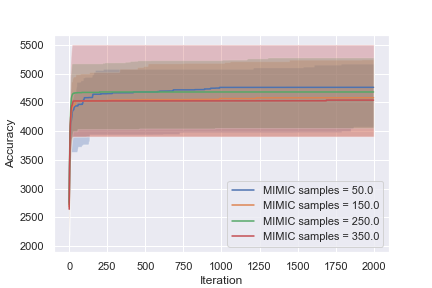
\includegraphics[width=\linewidth]{../graphics/tsp_MIMIC_Iteration_Error_MIMIC_samples.png}
						\caption{Accuracy on TSP with MIMIC, for different number of samples}
						\label{tsp:mimic_samples}
					\end{subfigure}
					~
					\begin{subfigure}[t]{0.45\columnwidth}
						\centering
						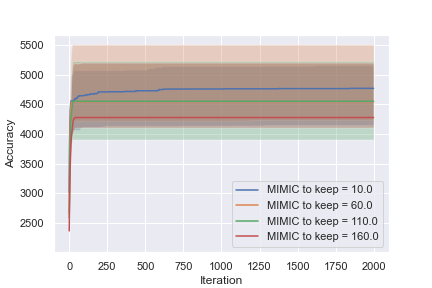
\includegraphics[width=\linewidth]{../graphics/tsp_MIMIC_Iteration_Error_MIMIC_to_keep.png}
						\caption{Accuracy on TSP with MIMIC, for different number of estimators kept, with a number of samples to 350}
						\label{tsp:mimic_to_keep}
					\end{subfigure}
					\caption{Accuracy of MIMIC on TSP according to the Number of Samples and the Number of Estimators Kept}
					\label{tsp:mimic}
				\end{figure}

				Let's discuss the impact of the number of samples generated for each iteration. We can see on figure \ref{tsp:mimic_samples} that the accuracy is the highest for low values of number of samples while it is the lowest for high values of number of samples. We can see that the best results are obtained with a number of samples of 50.

				On figure \ref{tsp:mimic_to_keep} we can see the impact of the number of samples to keep from an iteration to another with a number of samples of 350. I decided to use a high number of samples at each iteration to make the different number of samples to keep more significants. We can see that the best median accuracy is given with a number of samples to keep of 10. The worse accuracy is given for a number of sample to keep of 160. It is interesting to see that, in TSP, a performant MIMIC is one with few samples generated for each iteration as well as a few samples kept from an iteration to another to try to combine the good solutions.

				In terms of computation time, MIMIC gives the worst results compared to the other algorithms.

				Finally, MIMIC gave the best results on this problem at the cost of a long computation time.
		\subsection{Flip Flop Problem}
			\subsubsection*{Introduction}
				The Flip Flop problem is a problem where we have a binary vector of size $n$ and we want to find the vector that has the most consecutive bit alternations. The fitness function is the number of consecutive bit alternations in the vector.

				We present on figure \ref{ff:all} the accuracy and the time for the different algorithms on this problem. We can see that the best median accuracy is given by SA followed by MIMC. We chose a vector of 50 bit which mean that the best possible score is 49. SA and MIMIC manage sometimes to get that maximal score. GA stops at 48 while RHC does not exceed 43.

				\begin{figure}[h]
					\centering
					\begin{subfigure}[t]{0.45\columnwidth}
						\centering
						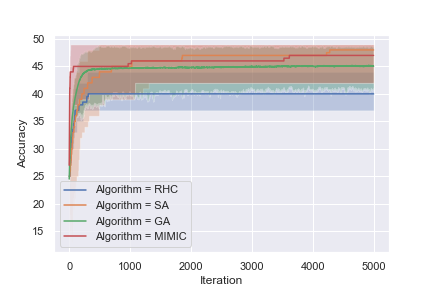
\includegraphics[width=\linewidth]{../graphics/flip_flop_all_Iteration_Error_Algorithm.png}
						\caption{Accuracy on Flip Flop problem for the different algorithms}
						\label{ff:all_accuracy}
					\end{subfigure}
					~
					\begin{subfigure}[t]{0.45\columnwidth}
						\centering
						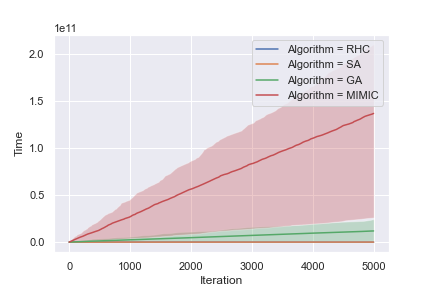
\includegraphics[width=\linewidth]{../graphics/flip_flop_all_Iteration_Time_Algorithm.png}
						\caption{Time on Flip Flop problem for the different algorithms}
						\label{ff:all_time}
					\end{subfigure}
					\caption{Accuracy and Time on Flip Flop Problem for the different algorithms}
					\label{ff:all}
				\end{figure}
			\subsubsection*{Randomised Hill Climbing}
				Again RHC does not success to perform well. We can see on figure \ref{ff:all_accuracy} that the best accuracy is given by a number of iterations bigger than 1000. But RHC does not success to improve even with much more iteration. It always get blocked on local optimums.

				In terms of computation time, RHC is the fastest algorithm of the four as we can see on figure \ref{ff:all_time}. Again that is explained by the simplicity of the algorithm.
			\subsubsection*{Simulated Annealing}
				In this problem, SA gives the best results. Figure \ref{ff:sa} shows the impact of the following parameters:
				\begin{itemize}
					\item Number of iterations
					\item Cooling rate
				\end{itemize}

				\begin{figure}[h]
					\begin{subfigure}[t]{0.45\columnwidth}
						\centering
						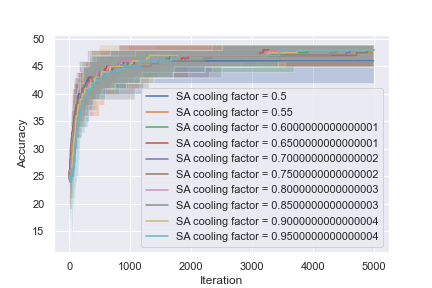
\includegraphics[width=\linewidth]{../graphics/flip_flop_SA_Iteration_Error_SA_cooling_factor.png}
						\caption{Accuracy on Flip Flop problem with SA, for different Cooling Factors}
						\label{ff:sa_cooling}
					\end{subfigure}
					~
					\begin{subfigure}[t]{0.45\columnwidth}
						\centering
						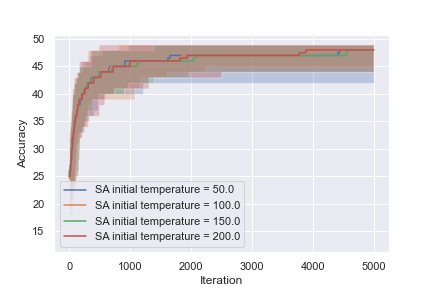
\includegraphics[width=\linewidth]{../graphics/flip_flop_SA_Iteration_Error_SA_initial_temperature.png}
						\caption{Accuracy on Flip Flop problem with SA, for different Initial Temperature}
						\label{ff:sa_initial_temp}
					\end{subfigure}
					\caption{Accuracy of SA on Flip Flop according to Initial Temperature and Cooling Factor}
					\label{ff:sa}
				\end{figure}

				We can see on figure \ref{ff:sa_cooling} that the best accuracy is given by a cooling factor of 0.95. The more the cooling factor is high, the more the accuracy seems to increase. That means that this problem works well with a temperature decreasing quickly.

				As we can wee on figure \ref{ff:sa_initial_temp}, the initial temperature does not really affect the accuracy of the SA optimizer.

				In terms of computation time, SA is the fastest algorithm of the four, with RHC, as we can see on figure \ref{ff:all_time}.

				To conclude, SA gives the best results on this problem with a fast computation time. It is perfectly suited for this problem. It is interesting to see the differencies of results between RHC and SA. Just by introducing some exploration as SA does, we can see that the results are much better.
			\subsubsection*{Genetic Algorithm}
				GA gives the second best results on this problem after SA and MIMIC. We can see on figure \ref{ff:ga} the impact of the following parameters:
				\begin{itemize}
					\item Population size
					\item Mutate Number
					\item Mate Number
				\end{itemize}

				\begin{figure}[h]
					\centering
					\begin{subfigure}[t]{0.32\columnwidth}
						\centering
						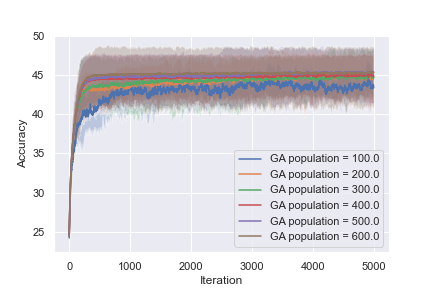
\includegraphics[width=\linewidth]{../graphics/flip_flop_GA_Iteration_Error_GA_population.png}
						\caption{Accuracy on Flip Flop problem with GA, for different population sizes}
						\label{ff:ga_pop}
					\end{subfigure}
					~
					\begin{subfigure}[t]{0.32\columnwidth}
						\centering
						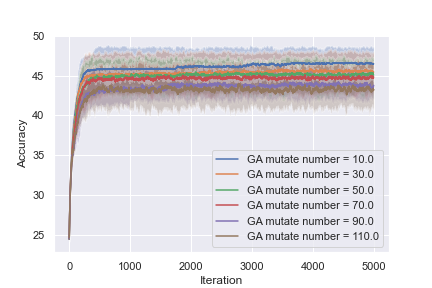
\includegraphics[width=\linewidth]{../graphics/flip_flop_GA_Iteration_Error_GA_mutate_number.png}
						\caption{Accuracy on Flip Flop problem with GA, for different mutate number, with population set to 600}
						\label{ff:ga_mutate}
					\end{subfigure}
					~
					\begin{subfigure}[t]{0.32\columnwidth}
						\centering
						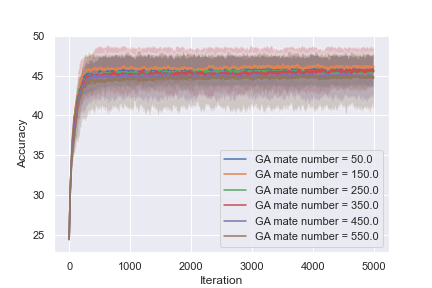
\includegraphics[width=\linewidth]{../graphics/flip_flop_GA_Iteration_Error_GA_mate_number.png}
						\caption{Accuracy on Flip Flop problem with GA, for different mate number, with population set to 600}
						\label{ff:ga_mate}
					\end{subfigure}
					\caption{Accuracy of GA on Flip Flop according to Population Size, Mutate Number and Mate Number}
					\label{ff:ga}
				\end{figure}

				We can see on figure \ref{ff:ga_pop} that the best accuracy is given by a population size of 600. The more the population size is high, the more the accuracy seems to increase. That means that this problem works well with a big population.

				The figure \ref{ff:ga_mutate} shows that the best accuracy is given by a mutate number of 10 and the worst by a mutate number of 110. Like in the previous problem, the optimiser works well with a small mutate number.

				Finally the figure \ref{ff:ga_mate} shows that the best accuracy is given by a mate number of 250. For that parameter it does not seem to have a linear impact on the accuracy. So finally the best optimisation for that problem is given by a relatively high population size (600), a small mutate number (10) and a mate number of 250.

				In terms of computation time, GA do not perform very well. It is the slowest algorithm after MIMIC, as we can see on figure \ref{ff:all_time}.
			\subsubsection*{MIMIC}
				MIMIC gives one of the best results on this problem with SA. We can see on figure \ref{ff:mimic} the impact of the following parameters:
				\begin{itemize}
					\item Number of samples
					\item Number of samples to keep
				\end{itemize}

				\begin{figure}[h]
					\centering
					\begin{subfigure}[t]{0.45\columnwidth}
						\centering
						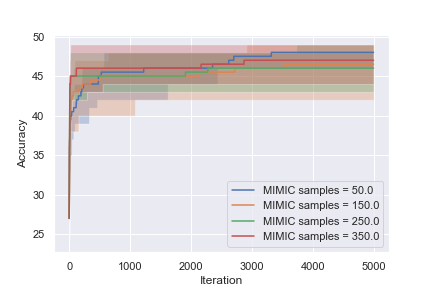
\includegraphics[width=\linewidth]{../graphics/flip_flop_MIMIC_Iteration_Error_MIMIC_samples.png}
						\caption{Accuracy on Flip Flop problem with MIMIC, for different number of samples}
						\label{ff:mimic_samples}
					\end{subfigure}
					~
					\begin{subfigure}[t]{0.45\columnwidth}
						\centering
						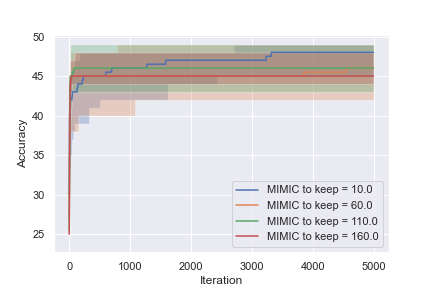
\includegraphics[width=\linewidth]{../graphics/flip_flop_MIMIC_Iteration_Error_MIMIC_to_keep.png}
						\caption{Accuracy on Flip Flop problem with MIMIC, for different number of estimators kept, with a number of samples set to 250}
						\label{ff:mimic_to_keep}
					\end{subfigure}
					\caption{Accuracy of MIMIC on Flip Flop according to Number of Samples and Number of Estimators Kept}
					\label{ff:mimic}
				\end{figure}

				We can see on figure \ref{ff:mimic_samples} that the best accuracy is given by a number of samples of 50. On figure \ref{ff:mimic_to_keep} we can see that the best accuracy is given by a number of estimators kept of 10. We have here the same results as in the previous problem.

				In terms of computation time, MIMIC is again the slowest algorithm of the four, as we can see on figure \ref{ff:all_time}.
		\subsection{Four Peaks Problem}
			\subsubsection*{Introduction}
				The Four Peaks problem is a problem with two local optima and two global optima. The local optima have wide basins of attraction while the global optima have narrow basins of attraction. The goal is to find the global optima. The function to optimise is defined as follows:
				\begin{equation}
					f(x, t) = tail(0, x) \uparrow (head(1, x) + r(x, t))
				\end{equation}
				Where:
				\begin{itemize}
					\item $x$ is the input vector, $x \in \{0, 1\}^n$
					\item $t$ is a threshold
					\item $head(k, x)$ is the number of leading $k$'s in $x$
					\item $tail(k, x)$ is the number of trailing $k$'s in $x$
				\end{itemize}
				and:
				\begin{equation}
					r(x, t) = \begin{cases}
						n & \text{if } tail(0, x) \geq t \land head(1, x) > t \\
						0 & \text{otherwise}
					\end{cases}
				\end{equation}

				We present on figure \ref{fp:all} the results of the four algorithms on this problem. We can see that the best accuracy is given by GA. GA is the only algorithm to manage to find the global optima. The other algorithms get stuck in a local optima.

				\begin{figure}[h]
					\centering
					\begin{subfigure}[t]{0.45\columnwidth}
						\centering
						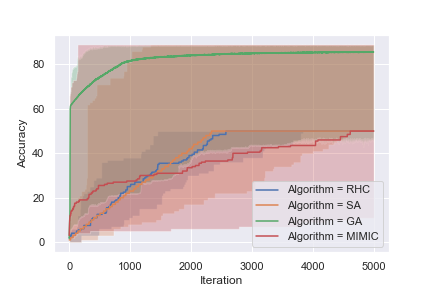
\includegraphics[width=\linewidth]{../graphics/four_peaks_all_Iteration_Error_Algorithm.png}
						\caption{Accuracy on Four Peaks problem for the different algorithms}
						\label{fp:all_accuracy}
					\end{subfigure}
					~
					\begin{subfigure}[t]{0.45\columnwidth}
						\centering
						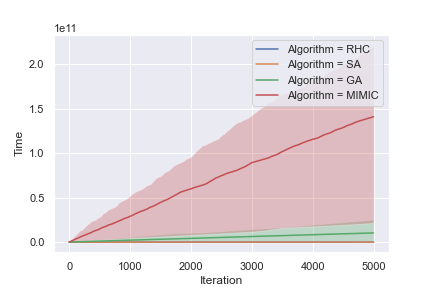
\includegraphics[width=\linewidth]{../graphics/four_peaks_all_Iteration_Time_Algorithm.png}
						\caption{Time on Four Peaks problem for the different algorithms}
						\label{fp:all_time}
					\end{subfigure}
					\caption{Accuracy and Time on Four Peaks Problem for the different algorithms}
					\label{fp:all}
				\end{figure}
			\subsubsection*{Randomised Hill Climbing}
				RHC goes not perform well on this problem. We can see on figure \ref{fp:all_accuracy} that it only finds the local optima. The fact that RHC does not explore the space of solutions is the reason why it does not find the global optima. We can see on figure \ref{fp:all_time} that RHC is the fastest algorithm of the four.
			\subsubsection*{Simulated Annealing}
				SA does not do much better that RHC. It sometimes manage to find the global optimum, but fails the most of the time. On figure \ref{fp:sa}, we can see that the colling factor as well as the initial temperature do not have a real impact on the accurace of SA. We can see on figure \ref{fp:all_time} that SA is the second fastest algorithm of the four. Unfortunately, even if SA introduce exploration compared to RHC, it does not manage to find the global optima most of the time. We will see that the crossover introduce by GA will give us better results.

				\begin{figure}[h]
					\centering
					\begin{subfigure}[t]{0.45\columnwidth}
						\centering
						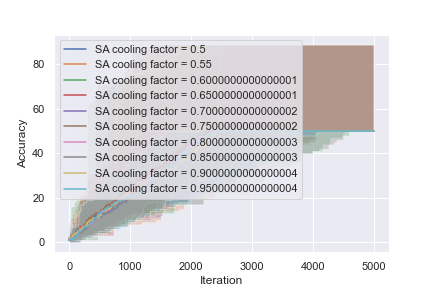
\includegraphics[width=\linewidth]{../graphics/four_peaks_SA_Iteration_Error_SA_cooling_factor.png}
						\caption{Accuracy on Four Peaks problem with SA, for different Cooling Factors}
						\label{fp:sa_cooling}
					\end{subfigure}
					~
					\begin{subfigure}[t]{0.45\columnwidth}
						\centering
						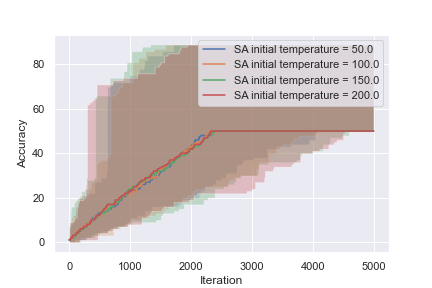
\includegraphics[width=\linewidth]{../graphics/four_peaks_SA_Iteration_Error_SA_initial_temperature.png}
						\caption{Accuracy on Four Peaks problem with SA, for different Initial temperatures}
						\label{fp:sa_initial_temp}
					\end{subfigure}
					\caption{Accuracy of SA on Four Peaks according to Cooling Factor and Initial Temperature}
					\label{fp:sa}
				\end{figure}
			\subsubsection*{Genetic Algorithm}
				GA is the only algorithm to manage to find the global optima. Let's the impact on the accuracy of the following parameters:
				\begin{itemize}
					\item Population Size
					\item Mutate Number
					\item Mate Number
				\end{itemize}

				\begin{figure}[h]
					\centering
					\begin{subfigure}[t]{0.32\columnwidth}
						\centering
						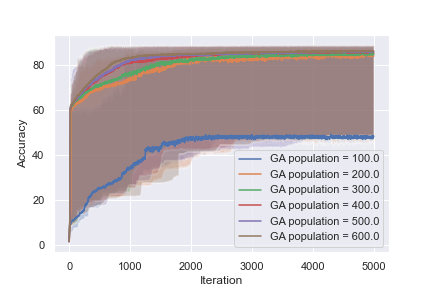
\includegraphics[width=\linewidth]{../graphics/four_peaks_GA_Iteration_Error_GA_population.png}
						\caption{Accuracy on Four Peaks problem with GA, for different population sizes}
						\label{fp:ga_pop}
					\end{subfigure}
					~
					\begin{subfigure}[t]{0.32\columnwidth}
						\centering
						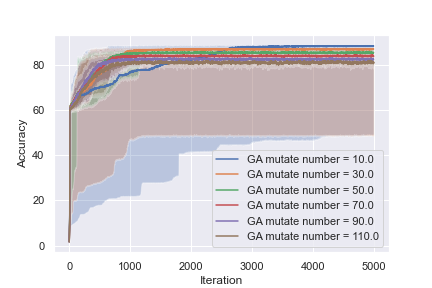
\includegraphics[width=\linewidth]{../graphics/four_peaks_GA_Iteration_Error_GA_mutate_number.png}
						\caption{Accuracy on Four Peaks problem with GA, for different mutate numbers, with population set to 600}
						\label{fp:ga_mutate}
					\end{subfigure}
					~
					\begin{subfigure}[t]{0.32\columnwidth}
						\centering
						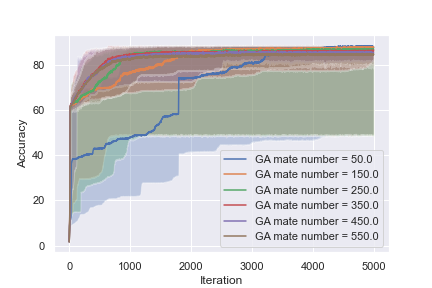
\includegraphics[width=\linewidth]{../graphics/four_peaks_GA_Iteration_Error_GA_mate_number.png}
						\caption{Accuracy on Four Peaks problem with GA, for different mate numbers, with population set to 600}
						\label{fp:ga_mate}
					\end{subfigure}
					\caption{Accuracy of GA on Four Peaks according to Population Size, Mutate Number and Mate Number}
					\label{fp:ga}
				\end{figure}

				We can see on figure \ref{fp:ga_pop} that the accuracy is heavely impacted by the population size. With a population size of 100, GA does not manage to find the global optima. With a population size above 200, it manages. But there is no real improvement with the different population sizes above 200. We can explain the fact that a small population size does not get good results by the fact that the population is not big enough to explore the space of solution and quickly get stuck on a local optima.

				Let's see the importance of the mutate number. We present the results on figure \ref{fp:ga_mutate} with a population size of 600. We can see as before that the best results are obtained with a small mutate number. We can explain this by the fact that a small mutate number will introduce more exploration in the population and will allow the population to get out of local optima.

				Finally, let's see the importance of the mate number. We present the results on figure \ref{fp:ga_mate} with a population size of 600. We can see that the mate number only impact the speed of convergence.

				In terms of time, we can see on figure \ref{fp:all_time} that GA is the slower than RHC and SA as always.

				In conclusion, GA is really well suited for this problem. It is the only algorithm to manage to find the global optima.
			\subsubsection*{MIMIC}
				MIMIC does not have better median result than RHC or SA. We can see the results of MIMIC on figure \ref{ff:all}. In this problem, The number of sample does not seem to have an impact on the accuracy of the optimiser. On the other side, the number of samples to keep plays a role. We can see the smallest one gives the better results while the larger one gives the worst results. We can explain this by the fact that the larger the number of samples to keep, the more the algorithm will be biased towards the best samples of the last iteration. In terms of computation time, MIMIC is the slowest algorithm of the four. Which makes it the worse algorithm for this problem.

				\begin{figure}[h]
					\centering
					\begin{subfigure}[t]{0.45\columnwidth}
						\centering
						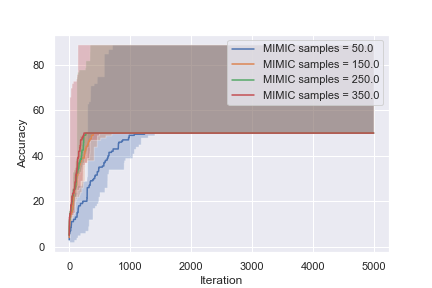
\includegraphics[width=\linewidth]{../graphics/four_peaks_MIMIC_Iteration_Error_MIMIC_samples.png}
						\caption{Accuracy on Four Peaks problem with MIMIC, for different number of samples}
						\label{fp:mimic_samples}
					\end{subfigure}
					~
					\begin{subfigure}[t]{0.45\columnwidth}
						\centering
						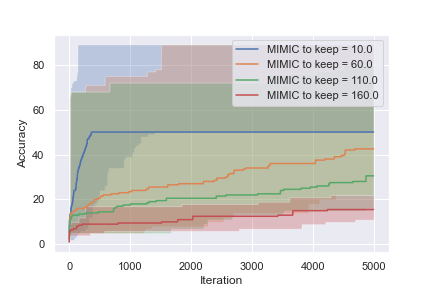
\includegraphics[width=\linewidth]{../graphics/four_peaks_MIMIC_Iteration_Error_MIMIC_to_keep.png}
						\caption{Accuracy on Four Peaks problem with MIMIC, for different number of estimator kept}
						\label{fp:mimic_to_keep}
					\end{subfigure}
					\caption{Accuracy of MIMIC on Four Peaks according to Number of Samples and Number of Estimators Kept}
					\label{fp:mimic}
				\end{figure}
		\subsection*{Conclusion}
			To conclude we saw the behaviour of the different algorithms on the different problems. We saw that RHC is the basic one. It gives poor results but is fast. SA is an improvement of RHC. It gives better results in general and is still as fast as RHC. GA and MIMIC are often the best optimisers. GA introduc the concept of population and crossover between iterations while MIMIC uses a probabilistic model to estimate the probability of a solution to be the best one which makes it the slower optimiser considered here.
	\section{Neural Networks}
		\subsection*{Introduction}
			In this section we will discuss the results of the randomised optimisation algorithms for training a neural network. There is some difference from the problems treated in the last section, mainly due to the supposed continuity of the weights in an artificial neural network. This can lead to issues when we want to to define a neighbor. The chosen solution adopted here is to update one weight by a random factor.

			The problem I have chosen to explore is the Gender dataset from the previous homework. The purpose of this dataset is to find the gender given some appearence characteritics. A more complete description of this dataset is available in homework 1.

			We will use the following notation for hidden layers: $n_1, n_2, n_3$ for a network with 3 hidden layers where $n_1$, $n_2$ and $n_3$ are the number of neurons in each layer respectively. The input and output are imposed by the dataset. The input layer is composed of 8 neurons. The output layer is composed of 1 neuron. The different networks tested are the following:
			\begin{itemize}
				\item $(5)$: 46 weights
				\item $(15)$: 163 weights
				\item $(35)$: 316 weights
				\item $(30,10)$: 561 weights
			\end{itemize}
			We can see on figure \ref{g:all} there is no need to seek for more complex networks.
			Adding new weight would only increase the computation time without improving the accuracy, and also may lead to overfitting.

			As an overview of the results, we can see that the best accuracy of 1.0 is find by each optimiser. One thing that is noticeable on \ref{g:all} is the fast variation on the curves. Those variations are not easy to explain as they are present with RHC algorithm which does not permit the result to decrease. One possible explaination would be that the plotted metric is not the same as the one used for training. In fact, the first is sum of squared errors while the second is the ratio between the number of correctly classified sample on the total number of sample. Thus, the accuracy probably fell down when the network learns that it's better not to be a bit wrong on every thing rather than being correct on the wanted value.

			Another thing to notice is that the training and the validation accuracy are very close. It could mean that the training and testing datasets are not independent. But we checked that it was not the case. So this means that the neural network is able to generalize to new data as well as it does not overfit. From now on, we will only display the validation accuracy on the figures as the curves are very similar to the training accuracy.

			In the next sections we will study more in depth the training process algorithm by algorithm.

			\begin{figure}[h]
				\centering
				\begin{subfigure}[t]{0.45\columnwidth}
					\centering
					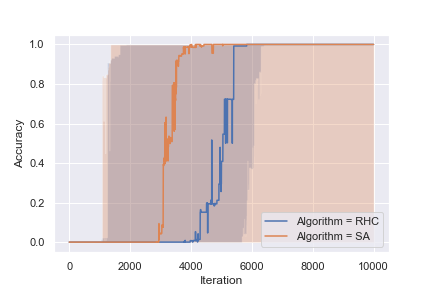
\includegraphics[width=\linewidth]{../graphics/g_all_Iteration_Error_Algorithm.png}
					\caption{Training accuracy on the Gender dataset for different algorithms}
					\label{g:all_test}
				\end{subfigure}
				~
				\begin{subfigure}[t]{0.45\columnwidth}
					\centering
					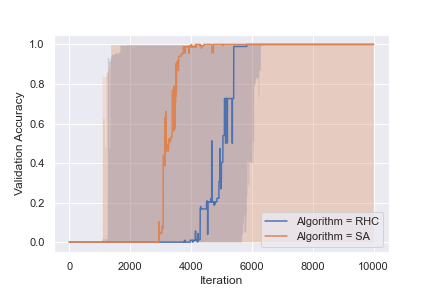
\includegraphics[width=1\linewidth]{../graphics/g_all_Iteration_Test_Error_Algorithm.png}
					\caption{Validation accuracy on the Gender dataset for different algorithms}
					\label{g:all_val}
				\end{subfigure}
				\caption{Training and Validation accuracy for the different training algorithms}
				\label{g:all}
			\end{figure}
		\subsection{Randomized Hill Climbing}
			We present on figure \ref{g:rhc} the results obtained with RHC. RHC succeeds to get the best accuracy on the validation set with all the different networks tested. The difference is the number of iteration required to converge. The best result is obtained with the network $(35)$ with an accuracy of 1.0 after only 1800 iterations. The worst result is obtained with the network $(30, 10)$ with an accuracy of 1.0 after 6200 iterations. An optimised network for that problem that gives a perfect iteration in the most efficient way is therefore the network $(35)$.

			RHC is again the fastest algorithm. It took approximately 1h to train all the different networks.

			\begin{figure}[h]
				\centering
				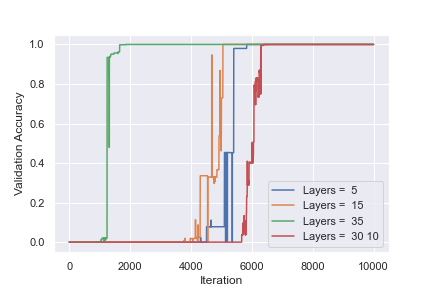
\includegraphics[width=0.45\linewidth]{../graphics/g_RHC_Iteration_Test_Error_Layers.png}
				\caption{Accuracy with RHC for different layers}
				\label{g:rhc}
			\end{figure}
		\subsection{Simulated Annealing}
			We present on figure \ref{g:sa} the results obtained with SA. SA also succeeds to get the best accuracy on the validation set. But that time not for all the networks. The best netwirk with RHC is the worst with SA. The network $(35)$ only manage to get an accuracy of 0.5 after 7000 iterations. The best result here is obtained with the network $(30, 10)$ with an accuracy of 1.0 after 4000 iterations. The other networks converge slower. I cannot really explain why the network $(35)$ is so bad with SA. It is possible that the network is too complex for the SA algorithm to find a good solution. The network $(30, 10)$ is the best network for that problem with SA.

			It took approximately 2h to train all the different networks with SA.

			\begin{figure}
				\centering
				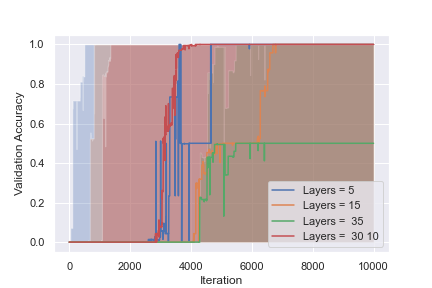
\includegraphics[width=0.45\linewidth]{../graphics/g_SA_Iteration_Test_Error_Layers.png}
				\caption{Accuracy with SA for different layers}
				\label{g:sa}
			\end{figure}
		\subsection{Genetic Algorithm}
			We present on figure \ref{g:ga} the results obtained with GA.

			\begin{figure}
				\centering
				% 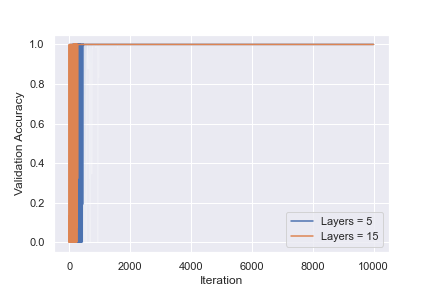
\includegraphics[width=0.7\linewidth]{../graphics/g_GA_Iteration_Test_Error_Layers.png}
				\caption{Accuracy with GA for different layers}
				\label{g:ga}
			\end{figure}
\end{document}